\documentclass[aspectratio=169]{beamer}
\usetheme{Madrid}
\usepackage{tikz}
\usepackage{fontawesome5}
\usepackage{graphicx}
\usepackage{amsmath}
\usepackage{xcolor}

% Color scheme - Democratic blue with gold accents
\definecolor{mainblue}{RGB}{25, 55, 135}
\definecolor{accentgold}{RGB}{255, 193, 7}
\definecolor{lightblue}{RGB}{66, 133, 244}
\definecolor{darkgray}{RGB}{45, 45, 45}
\definecolor{white}{RGB}{255, 255, 255}

\setbeamercolor{palette primary}{bg=mainblue,fg=white}
\setbeamercolor{palette secondary}{bg=lightblue,fg=white}
\setbeamercolor{palette tertiary}{bg=accentgold,fg=darkgray}
\setbeamercolor{structure}{fg=mainblue}
\setbeamercolor{title}{fg=white}
\setbeamercolor{frametitle}{bg=mainblue,fg=white}
\setbeamercolor{block title}{bg=lightblue,fg=white}
\setbeamercolor{block body}{bg=lightblue!10}

% Remove navigation symbols
\setbeamertemplate{navigation symbols}{}

% Custom footer
\setbeamertemplate{footline}{
  \leavevmode%
  \hbox{%
  \begin{beamercolorbox}[wd=.33\paperwidth,ht=2.5ex,dp=1ex,center]{palette primary}%
    \usebeamerfont{author in head/foot}\insertshortauthor
  \end{beamercolorbox}%
  \begin{beamercolorbox}[wd=.34\paperwidth,ht=2.5ex,dp=1ex,center]{palette secondary}%
    \usebeamerfont{title in head/foot}\insertshorttitle
  \end{beamercolorbox}%
  \begin{beamercolorbox}[wd=.33\paperwidth,ht=2.5ex,dp=1ex,right]{palette tertiary}%
    \usebeamerfont{date in head/foot}\insertframenumber{} / \inserttotalframenumber\hspace*{2ex}
  \end{beamercolorbox}}%
  \vskip0pt%
}

% Title information
\title{\textbf{SPY DAO}}
\subtitle{Democratizing Corporate Governance for Index Investors}
\author{Built for Rails Hackathon}
\date{\today}

\begin{document}

% Title Slide
{
\setbeamercolor{background canvas}{bg=mainblue}
\begin{frame}
\vspace{1cm}
\begin{center}
    {\Huge\textcolor{white}{\textbf{SPY DAO}}}
    
    \vspace{0.5cm}
    {\Large\textcolor{accentgold}{Democratizing Corporate Governance}}
    
    \vspace{0.3cm}
    {\large\textcolor{white}{for Index Investors}}
    
    \vspace{1.5cm}
    
\begin{tikzpicture}
        \fill[accentgold] (0,0) circle (0.8cm);
        \node[white] at (0,0) {\Huge\faVoteYea};
    \end{tikzpicture}
    
    \vspace{1cm}
    {\small\textcolor{white}{Built for Rails Hackathon}}
\end{center}
\end{frame}
}

% Slide 1: Unlocking Trillions
\begin{frame}{Unlocking Trillions}
\vspace{0.5cm}
\begin{center}
    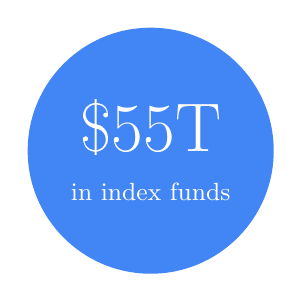
\begin{tikzpicture}
        \node[circle,fill=lightblue,text=white,minimum size=3cm] at (0,0) {
            \begin{minipage}{2.5cm}
                \centering
                {\Huge\$55T}\\[0.2cm]
                {\small in index funds}
            \end{minipage}
        };
    \end{tikzpicture}
    
    \vspace{1cm}
    {\Large\textcolor{mainblue}{\textbf{Zero voting power}}}
    
    \vspace{0.5cm}
    {\large Unlock corporate influence at scale}
\end{center}
\end{frame}

% Slide 2: Participate in 500 Companies
\begin{frame}{Participate in 500 Companies}
\vspace{0.3cm}
\begin{center}
    {\LARGE\textcolor{mainblue}{\textbf{S\&P 500}}}
    
    \vspace{0.8cm}
    
\begin{tikzpicture}
        \foreach \i in {1,...,15} {
            \pgfmathsetmacro{\angle}{360/15*\i}
            \pgfmathsetmacro{\radius}{2}
            \fill[lightblue] ({\radius*cos(\angle)},{\radius*sin(\angle)}) circle (0.2cm);
        }
        \node[circle,fill=accentgold,text=white,minimum size=1.5cm] at (0,0) {
            \textbf{YOU}
        };
    \end{tikzpicture}
    
    \vspace{0.8cm}
    {\Large One deposit. Complete market access.}
\end{center}
\end{frame}

% Slide 3: Verified Share Purchases
\begin{frame}{Verified Share Purchases}
\vspace{0.5cm}
\begin{center}
    \begin{tikzpicture}[scale=1.2]
        % Blockchain
        \foreach \x in {0,1.5,3} {
            \draw[fill=lightblue,draw=mainblue,thick] (\x,0) rectangle (\x+1.2,1.2);
            \node[white] at (\x+0.6,0.6) {\faLink};
        }
        
        % Arrow down
        \draw[->,ultra thick,accentgold] (2,-0.5) -- (2,-1.5);
        
        % Real shares
        \draw[fill=accentgold,draw=mainblue,thick] (0.5,-2) rectangle (3.5,-3);
        \node[white] at (2,-2.5) {\Large\faCertificate\ Real Shares};
    \end{tikzpicture}
    
    \vspace{0.5cm}
    {\Large\textbf{On-chain oracle + API bridge}}
    
    \vspace{0.3cm}
    {\large Copy-trade the SPY with proof}
\end{center}
\end{frame}

% Slide 4: ERC-4626 Governance
\begin{frame}{ERC-4626 Governance}
\vspace{0.5cm}
\begin{center}
    {\Huge\textcolor{mainblue}{\texttt{ERC-4626}}}
    
    \vspace{0.8cm}
    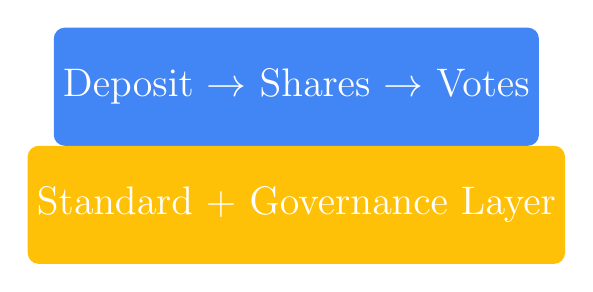
\begin{tikzpicture}
        \node[rectangle,fill=lightblue,text=white,minimum width=6cm,minimum height=1.5cm,rounded corners] at (0,1) {
            \Large Deposit $\rightarrow$ Shares $\rightarrow$ Votes
        };
        
        \node[rectangle,fill=accentgold,text=white,minimum width=6cm,minimum height=1.5cm,rounded corners] at (0,-0.5) {
            \Large Standard + Governance Layer
        };
    \end{tikzpicture}
    
    \vspace{0.8cm}
    {\large Programmable corporate democracy}
\end{center}
\end{frame}

% Slide 5: Deposits at Internet Scale
\begin{frame}{Deposits at Internet Scale}
\vspace{0.5cm}
\begin{center}
    
\begin{tikzpicture}
        % Globe in center
        \fill[lightblue] (0,0) circle (1.5cm);
        \node[white] at (0,0) {\Huge\faGlobe};
        
        % Arrows pointing inward
        \foreach \angle in {0,60,120,180,240,300} {
            \draw[->,ultra thick,accentgold] ({\angle+20}:3cm) -- ({\angle+20}:1.8cm);
            \fill[mainblue] (\angle:3cm) circle (0.15cm);
        }
    \end{tikzpicture}
    
    \vspace{0.8cm}
    {\Large\textbf{Permissionless. Borderless. Instant.}}
    
    \vspace{0.3cm}
    {\large Global capital meets corporate governance}
\end{center}
\end{frame}

% Slide 6: Delegated Voting Power
\begin{frame}{Delegated Voting Power}
\vspace{0.5cm}
\begin{center}
    \begin{tikzpicture}
        % Multiple users
        \foreach \x in {-3,-1.5,0,1.5,3} {
            \fill[lightblue] (\x,2) circle (0.3cm);
            \node[white] at (\x,2) {\small\faUser};
        }
        
        % Arrows converging
        \foreach \x in {-3,-1.5,0,1.5,3} {
            \draw[->,thick,mainblue] (\x,1.5) -- (0,0.2);
        }
        
        % DAO
        \node[circle,fill=accentgold,text=white,minimum size=2cm] at (0,-0.5) {
            \begin{minipage}{1.8cm}
                \centering
                \textbf{SPY}\\
                \textbf{DAO}
            \end{minipage}
        };
    \end{tikzpicture}
    
    \vspace{0.5cm}
    {\Large Your shares. Your voice. Our power.}
\end{center}
\end{frame}

% Slide 7: Aggregated Authority
\begin{frame}{Aggregated Authority}
\vspace{0.5cm}
\begin{center}
    {\Huge\textcolor{mainblue}{\textbf{1 + 1 + 1 = POWER}}}
    
    \vspace{1cm}
    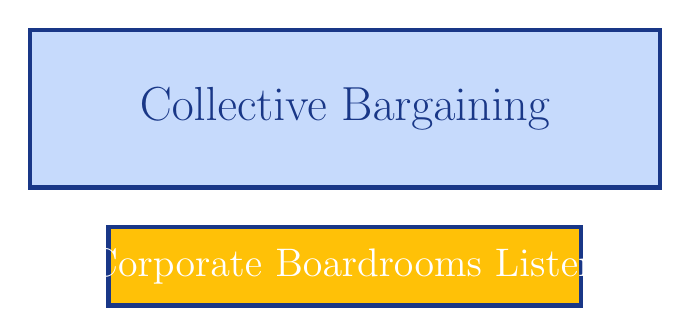
\begin{tikzpicture}
        \draw[fill=lightblue!30,draw=mainblue,ultra thick] (-4,0) rectangle (4,2);
        \node[mainblue] at (0,1) {\LARGE Collective Bargaining};
        
        \draw[fill=accentgold,draw=mainblue,ultra thick] (-3,-1.5) rectangle (3,-0.5);
        \node[white] at (0,-1) {\Large Corporate Boardrooms Listen};
    \end{tikzpicture}
    
    \vspace{0.8cm}
    {\large Retail investors become institutional force}
\end{center}
\end{frame}

% Slide 8: Broker-Based Ownership
\begin{frame}{Broker-Based Ownership}
\vspace{0.5cm}
\begin{center}
    \begin{tikzpicture}
        % Old way - crossed out
        \draw[fill=lightblue!20,draw=mainblue,dashed] (-5,1) rectangle (-1,2.5);
        \node[mainblue] at (-3,1.75) {You $\rightarrow$ Broker $\rightarrow$ \faTimes};
        \draw[red,ultra thick] (-5.5,0.8) -- (-0.5,2.7);
        
        % New way
        \draw[fill=accentgold,draw=mainblue,ultra thick] (1,1) rectangle (5,2.5);
        \node[white] at (3,1.75) {You $\rightarrow$ SPY DAO $\rightarrow$ \faCheck};
    \end{tikzpicture}
    
    \vspace{1cm}
    {\Large\textbf{Custody without compromise}}
    
    \vspace{0.5cm}
    {\large Real ownership. Real representation.}
\end{center}
\end{frame}

% Slide 9: Earn Governance Yields
\begin{frame}{Earn Governance Yields}
\vspace{0.5cm}
\begin{center}
    \begin{tikzpicture}
        % Stack of benefits
        \node[rectangle,fill=lightblue,text=white,minimum width=8cm,minimum height=1.2cm,rounded corners] at (0,2) {
            \Large\faChartLine\ SPY Market Returns
        };
        
        \node[rectangle,fill=accentgold,text=white,minimum width=8cm,minimum height=1.2cm,rounded corners] at (0,0.5) {
            \Large\faVoteYea\ Governance Participation Rewards
        };
        
        \node[rectangle,fill=mainblue,text=white,minimum width=8cm,minimum height=1.2cm,rounded corners] at (0,-1) {
            \Large\faTrophy\ Democracy in Action
        };
    \end{tikzpicture}
    
    \vspace{0.8cm}
    {\large Incentivized engagement = Better outcomes}
\end{center}
\end{frame}

% Slide 10: Index Investing and Control
\begin{frame}{Index Investing + Control}
\vspace{0.5cm}
\begin{center}
    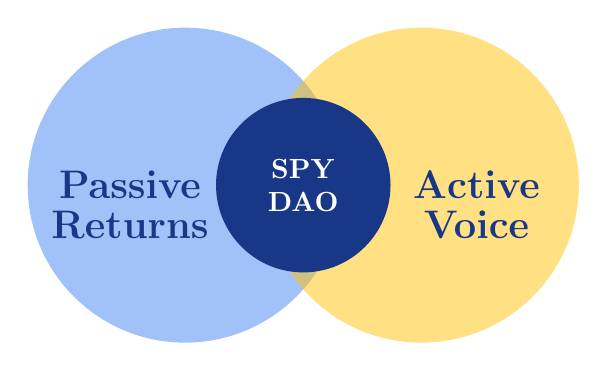
\begin{tikzpicture}
        % Venn diagram
        \fill[lightblue,opacity=0.5] (-1.5,0) circle (2cm);
        \fill[accentgold,opacity=0.5] (1.5,0) circle (2cm);
        
        \node[mainblue] at (-2.2,0) {\Large\textbf{Passive}};
        \node[mainblue] at (-2.2,-0.5) {\Large\textbf{Returns}};
        
        \node[mainblue] at (2.2,0) {\Large\textbf{Active}};
        \node[mainblue] at (2.2,-0.5) {\Large\textbf{Voice}};
        
        \node[white,circle,fill=mainblue,minimum size=2cm] at (0,0) {
            \begin{minipage}{1.8cm}
                \centering
                \textbf{SPY}\\
                \textbf{DAO}
            \end{minipage}
        };
    \end{tikzpicture}
    
    \vspace{0.8cm}
    {\Large Best of both worlds}
\end{center}
\end{frame}

% Slide 11: Returning Voting Rights
\begin{frame}{Returning Voting Rights to the People}
\vspace{0.3cm}
\begin{center}
    
\begin{tikzpicture}
        % Hand holding up vote
        \fill[accentgold] (0,0) -- (-1,-2) -- (-0.5,-2.2) -- (0,-1) -- (0.5,-2.2) -- (1,-2) -- cycle;
        \fill[lightblue] (0,0) circle (1.2cm);
        \node[white] at (0,0) {\Huge\faVoteYea};
    \end{tikzpicture}
    
    \vspace{0.8cm}
    {\Huge\textcolor{mainblue}{\textbf{Power to the People}}}
    
    \vspace{0.5cm}
    {\Large Corporate democracy restored}
    
    \vspace{0.3cm}
    {\large One token = One vote = Real change}
\end{center}
\end{frame}

% Slide 12: Permissionless Global Economic Access
\begin{frame}{Permissionless Global Economic Access}
\vspace{0.5cm}
\begin{center}
    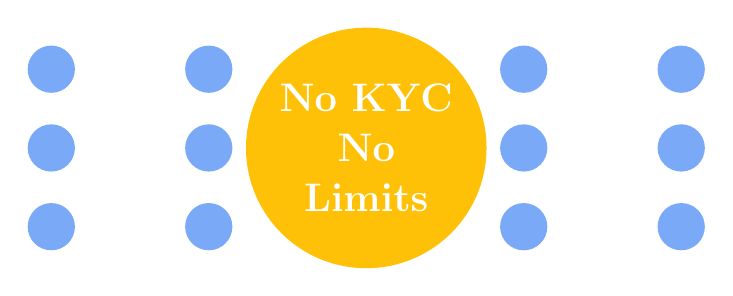
\begin{tikzpicture}
        % World map style representation
        \foreach \x in {-4,-2,0,2,4} {
            \foreach \y in {-1,0,1} {
                \fill[lightblue,opacity=0.7] (\x,\y) circle (0.3cm);
            }
        }
        
        % Central node
        \node[circle,fill=accentgold,text=white,minimum size=2.5cm] at (0,0) {
            \begin{minipage}{2.2cm}
                \centering
                \Large\textbf{No KYC}\\
                \Large\textbf{No Limits}
            \end{minipage}
        };
    \end{tikzpicture}
    
    \vspace{0.8cm}
    {\Large\textbf{Financial inclusion meets corporate governance}}
    
    \vspace{0.3cm}
    {\large Anyone, anywhere, anytime}
\end{center}
\end{frame}

% Call to Action Slide
{
\setbeamercolor{background canvas}{bg=mainblue}
\begin{frame}
\vspace{0.5cm}
\begin{center}
    {\Huge\textcolor{accentgold}{\textbf{Join the Revolution}}}
    
    \vspace{1cm}
    \begin{tikzpicture}
        \node[rectangle,fill=accentgold,text=white,minimum width=10cm,minimum height=1.5cm,rounded corners] at (0,1.5) {
            \Large\faRocket\ Deposit. Vote. Govern.
        };
        
        \node[rectangle,fill=white,text=mainblue,minimum width=10cm,minimum height=1.5cm,rounded corners] at (0,0) {
            \Large\faUsers\ Build SPY DAO with us
        };
        
        \node[rectangle,fill=lightblue,text=white,minimum width=10cm,minimum height=1.5cm,rounded corners] at (0,-1.5) {
            \Large\faGlobe\ Democratize corporate America
        };
    \end{tikzpicture}
    
    \vspace{1cm}
    {\Large\textcolor{white}{\textbf{spydao.finance}}}
    
    \vspace{0.3cm}
    {\small\textcolor{white}{Built for Rails Hackathon}}
\end{center}
\end{frame}
}

\end{document}
